\newpage
\begin{center}
\textbf{\large 3. ВЫЧИСЛИТЕЛЬНЫЙ ЭКСПЕРИМЕНТ}
\end{center}
\refstepcounter{chapter}
\addcontentsline{toc}{chapter}{3. ВЫЧИСЛИТЕЛЬНЫЙ ЭКСПЕРИМЕНТ}


В рамках данной главы будет рассмотрен процесс создания тестовых наборов данных, разработка алгоритма распределения преподавателей и учеников, а также его тестирование на практике. Полученные результаты будут проанализированы с целью оценки эффективности предложенного подхода и его применимости в реальных условиях образовательной деятельности.

Ключевые аспекты данной главы включают в себя:
\begin{itemize}
    \item Создание тестовых наборов данных, включающих информацию о преподавателях, аудиториях и учениках.
    \item Разработка и реализация алгоритма распределения преподавателей по аудиторно-временным слотам.
    \item Тестирование алгоритма на сгенерированных тестовых данных и анализ полученных результатов.
    \item Исследование эффективности алгоритма и его применимость в реальных условиях образовательной практики.
\end{itemize}

\section{Тестирование алгоритма на тестовом наборе данных}
\label{MACR-SecIntroduction}
\subsection{Создание тестовых наборов данных}
\label{PRIMe-SubSecDBSCAN}
Создан алгоритм для генерации тестовых наборов данных. Набор данных состоит из 3х сущностей:Преподаватель ~\ref{data1}, Аудитория ~\ref{data2} и Ученик ~\ref{data3}. В тестовом наборе данных количество преподавателей варьировалось от 10 до 20, каждый из которых обладает уникальными характеристиками, включая имя, предмет преподавания, класс обучения, желаемое время занятий. Количество учеников меняется  от 250 до 450 и  описывается такими параметрами, как имя, предмет обучения, класс, желаемое время занятий и ценность ученика.Верхняя и нижняя границы количества аудиторий соответственно равны  20 и 10 для занятий по математике и 15 и 10 для занятий по информатике, куборо. Каждая аудитория имеет свой уникальный номер, предмет, время доступности и количество свободных мест.
\begin{figure}[!ht]
  \centering
  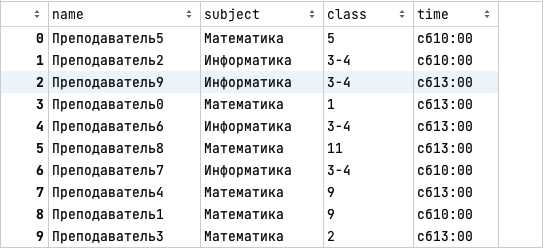
\includegraphics[width=\linewidth]{Images/data_1.png}
  \caption{\textbf{Пример данных преподавателей.}}
  \label{data1}
\end{figure}
\begin{figure}[!ht]
  \centering
  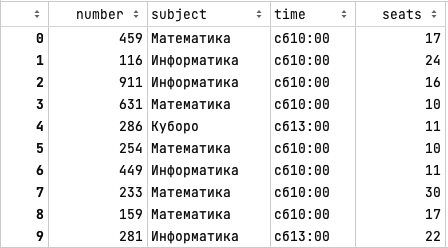
\includegraphics[width=\linewidth]{Images/data_2.png}
  \caption{\textbf{Пример данных аудиторий.}}
  \label{data2}
\end{figure} 
\begin{figure}[!ht]
  \centering
  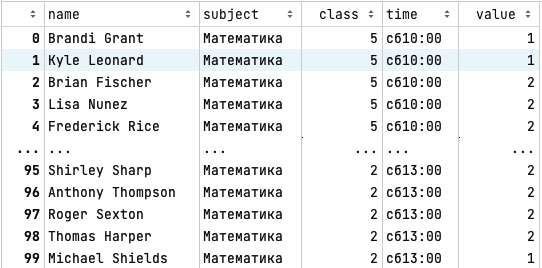
\includegraphics[width=\linewidth]{Images/data_3.png}
  \caption{\textbf{Пример данных учеников.}}
  \label{data3}
\end{figure}

\subsection{Работа алгоритма составления расписания и назначения учеников в расписание}
\label{PRIMe-SubSecDBSCAN}
После создания тестовых наборов данных преподаватели распределяются по аудиторно-временным слотам ~\ref{dist_1}. Распределение происходит в зависимости от спроса на преподавателя(по возрастанию количества занятий у преподавателя).\begin{figure}[!ht]
  \centering
  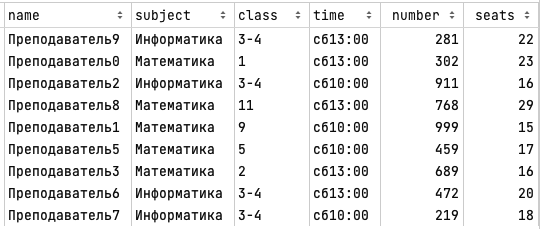
\includegraphics[width=\linewidth]{Images/dist_1.png}
  \caption{\textbf{Пример результата распределения по аудиторно-временным слотам.}}
  \label{dist_1}
\end{figure}

Назначение учеников в расписание происходит на основе спроса на предмет и на основании ценности ученика ~\ref{dist_3}. Ученики не попавшие в расписание назначаются в группу резерва~\ref{dist_2}
\begin{figure}[!ht]
  \centering
  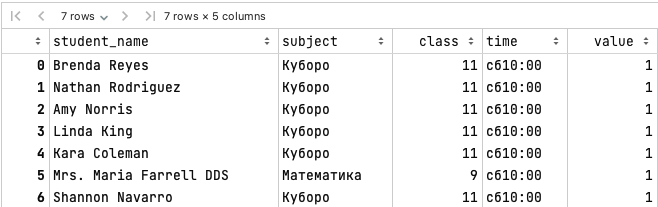
\includegraphics[width=\linewidth]{Images/dist_3.png}
  \caption{\textbf{Результат распределения учеников по аудиторно-временным слотам.}}
  \label{dist_3}
\end{figure}
\begin{figure}[!ht]
  \centering
  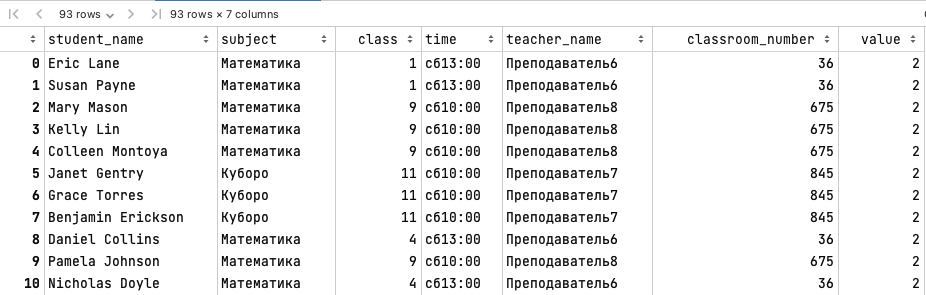
\includegraphics[width=\linewidth]{Images/dist_2.png}
  \caption{\textbf{Результат назначения учеников в группу резерва.}}
  \label{dist_2}
\end{figure}




В рамках исследования было решено 100 задач на сгенерированных данных с целью оценки ее эффективности. Результаты вычислительного эксперимента показывают, что в среднем 19.5 преподавателей из 20 были успешно распределены по аудиторно-временным слотам.  Было замечено, что в среднем 77.09 - 79,72 \% из 400 учеников были распределены по слотам преподаватель-аудитория (см. рис. 5, 6, 7), что свидетельствует о высокой эффективности алгоритма.\begin{figure}[!ht]
  \centering
  \begin{subfigure}[b]{0.45\textwidth}
    \centering
    \includegraphics[width=\textwidth]{Images/stat_1.png}
    \caption{Вывод метрик по возрастанию количества  слотов преподавателя.}
    \label{fig:stat1}
  \end{subfigure}
  \hfill
  \begin{subfigure}[b]{0.45\textwidth}
    \centering
    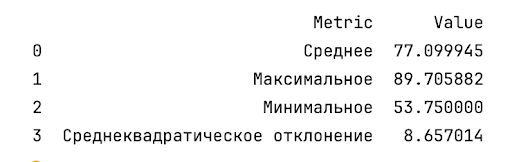
\includegraphics[width=\textwidth]{Images/stat_2.png}
    \caption{Вывод метрик по убыванию количества  слотов преподавателя}
    \label{fig:stat2}
  \end{subfigure}
  \caption{Статистика результатов}
  \label{fig:both_images}
\end{figure}


\section{Тестирование алгоритма на наборе данных профориентационной школы}
\label{MACR-SecMethods}

\subsection{Нормализация набора данных}
\label{MACR-SubSecMD}

Для нормализации  были получены исходные данные в виде набора файлов формата .xlsx, которые содержали такие поля как: Отметка времени, Фамилия ученика, Имя ученика, Отчество ученика, Дата рождения ученика, Адрес ученика с индексом, Школа, Адрес электронной почты ученика (если есть), Телефон ученика (если есть), Фамилия родителя, Имя родителя, Отчество родителя, Дата рождения родителя, Адрес родителя с индексом, Адрес электронной почты родителя, Телефон родителя, Будете ли заниматься в этом году в группах по информатике?, Согласие на обработку персональных данных, Примечания, Адрес электронной почты. //перечислением
Все файлы можно разделить на 3 категории: записи по информатике, записи по математике и записи для формирования новых дополнительных групп. Из особенностей данных можно выделить то, что они не приведены к одному виду. По математике и информатике данные имеют разные поля, поле примечание содержит не конкретную информацию, плохо поддающуюся обработке. Поле “Школа” имеет нетипизированный вид.
Изначально данные всех файлов были объединены в одну таблицу. Создан алгоритм приведения школ к одному виду, удаление дубликатов данных. Приведение поля примечания к одному виду(наличие желаемого временного слота). Создана база данных аудиторий и преподавателей

\subsection{Изменение формы регистрации для обучения }
\label{MACR-SubSecMD}

В связи с тем, что данные на этапе заполнения форм не были приведены к единому виду, сформулированы предложения по улучшению существующих регистрационных форм учащихся. Для этого в поле “Школа” были собраны школы обучающихся при помощи отдельной программы парсинга с сайта \href{https://admomsk.ru/web/guest/1132}{https://admomsk.ru/web/guest/1132}. После парсинга результатом программы стал файл xlsx с названиями всех школ. В формы записи учеников был добавлен список с выбором той или иной школы. Также было переработано поле “Номер телефона” и “email” с помощью регулярных выражений. Были введены обязательные поля: Фамилия, Имя, Фамилия родителя, Имя родителя, Отчество родителя, Школа.

\subsection{Тестирование на приведенных данных}
\label{MACR-SubSecMD}
Результаты вычислительного эксперимента на данных 2021-2022 года показывают, что в среднем 40 преподавателей из 42 были успешно распределены по аудиторно-временным слотам.  Было замечено, что в среднем 350 из 415 учеников были распределены по слотам преподаватель-аудитория. Результаты были неудовлетворительные, после проверки данных, оказалось что входные данные не до конца обработаны, были приняты действия по приведению и дополнению данных профориентационной школы.После обработки данных в среднем 401 ученик из 415 учеников были распределены по аудиторно временным слотам.






\section{Заключение главы}
\label{MACR-SecConclusions}

В рамках данной главы исследовано влияние формы данных на эффективность алгоритма. Проведенные вычислительные эксперименты показали высокую эффективность алгоритма при различных наборах данных, что подтверждает его применимость в реальных условиях.
